% !TEX root=../thesis.tex

\chapter{Research and Method} % (fold)
% Research questions and method
\label{cha:research_questions_and_method}

\section{Research Method} % (fold)
\label{sec:research_method}

During the work of this thesis, the Design science research process (DSRP) was
followed as the research method. 
This is based around 6 steps which is presented in the list
below and can be seen in \Ref{fig:DSRP}. Depending on what the focus of the project is, the project can start at
almost any of the steps below.\cite{peffers2006design}

\begin{description}
	\item [1. Problem identification and motivation] Defines the problem to be
	researched. 
	\item [2. Objectives of a solution] Infer the goals of the solution.
	\item [3. Design and development] Creates a artifact for the solution.
	\item [4. Demonstration] Demonstrate the created artifact.
	\item [5. Evaluation] Observe and measure how the artifact gives a solution 
	to the problem.
	\item [6. Communication] Communicate the problem along with the artifact.
\end{description}


This process loop is typically iterated a number of times before the final
design artifact is generated. Each time the evaluation is
performed, it then provides feedback information and a better understanding of
the problem in order to the quality of the product.\cite{von2004design}

\begin{figure}[!htbp]
	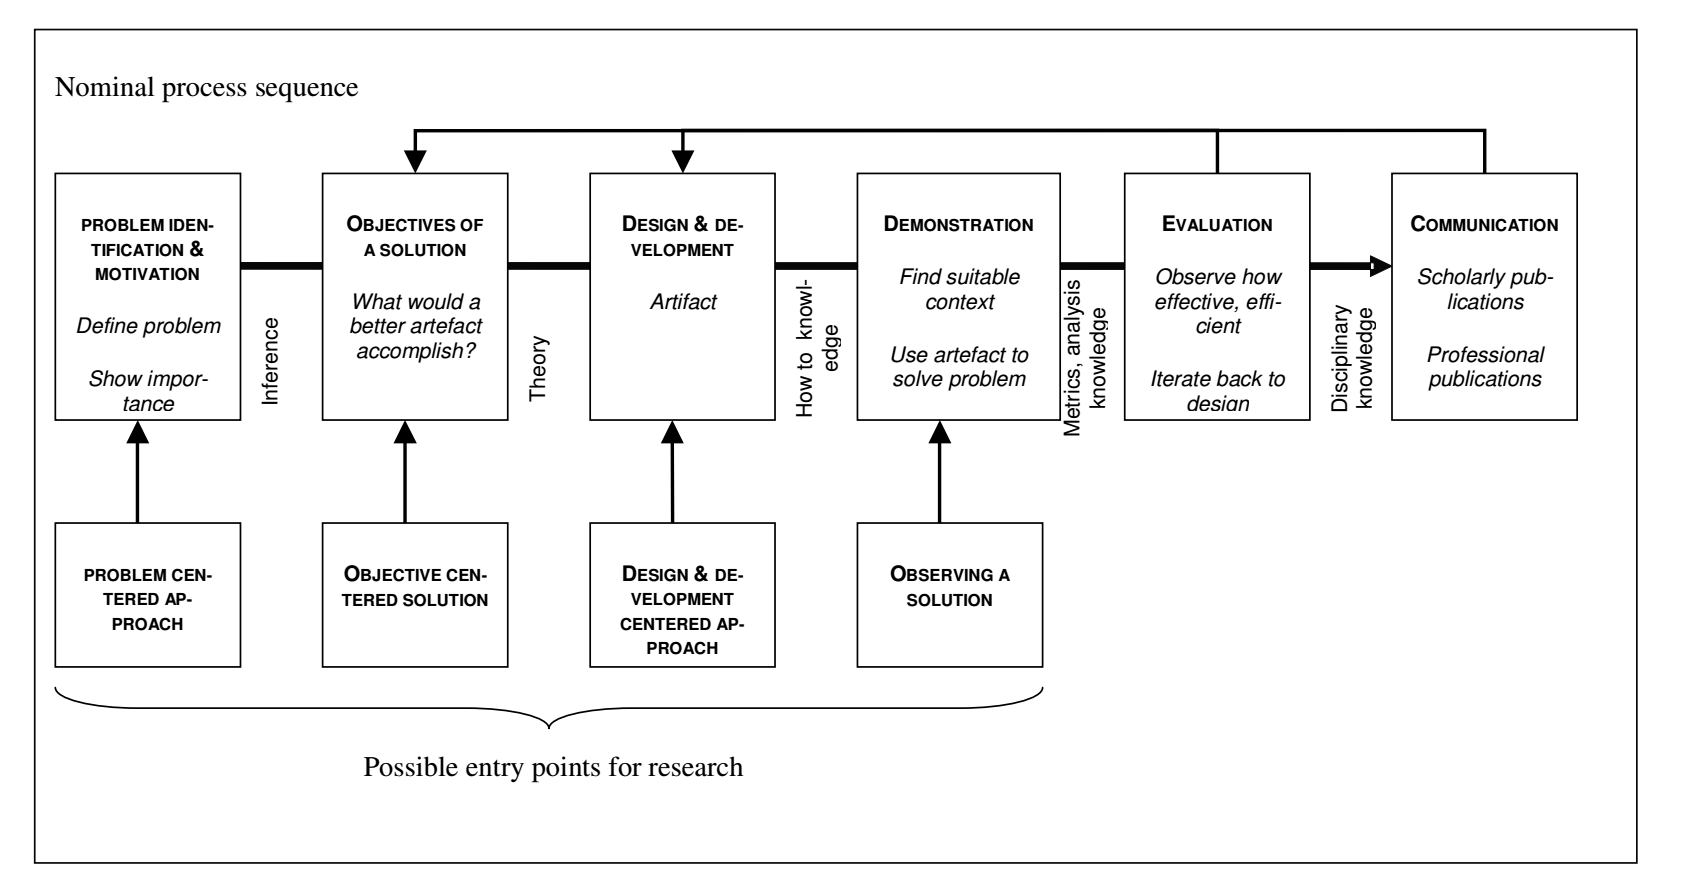
\includegraphics[width=\textwidth,center]{dsrp_modell.png}
	\caption[Design science research process (DSRP) model]{Design research process (DSRP)
	model\cite{peffers2006design}}
	\label{fig:DSRP}
\end{figure}


% section research_method (end)

\section{Research} % (fold)
\label{sec:workshops}
Since the research problem was given at the start of the thesis, a natural
starting point was at step 2 of the DSRP. At first a case study of similar 
systems was performed. These systems where then categorized into frameworks to 
cover the functionality and what information was presented. Based on these 
frameworks, the initial goals were defined.

The second step performed of defining the goals of the solution and the
prototype was to have two workshops. These workshops were meant to further 
define the needs of the stakeholders and define the goals for the prototype.
Participating on these workshops were several stakeholders which helped define
the direction of the process.

As part of the iterative loop, a meeting with the supervisors were held each 
week where the continued development of a prototype was demonstrated and 
evaluated against the objectives of the solution. Based on the evaluation that 
took place during these meetings, the process was returned to step 2 or 3 
where the objectives and design were looked at again and optimally redefined.

% section workshops (end)

% chapter research_questions_and_method (end)

